\documentclass[12pt]{article}
\usepackage{graphicx}
\usepackage{graphics}
\usepackage[percent]{overpic}
\usepackage{hyperref}
\usepackage{indentfirst}
\renewcommand\theequation{{\color{red}\arabic{equation}}}
\hypersetup{colorlinks=true}
\usepackage{amsmath}
\usepackage{amsfonts}
\usepackage{float}
\usepackage{algorithm}
\usepackage{algorithmic}
\usepackage{caption}
\usepackage{subfigure}
%\usepackage{subcaption}
\usepackage[numbers]{natbib}
\bibliographystyle{plainnat}%{ieeetr}%Choose a bibliograhpic style
\usepackage[toc,page]{appendix}
\addtolength{\textwidth}{1.1in}
\addtolength{\hoffset}{-0.5in}
\addtolength{\textheight}{1.1in}
\addtolength{\voffset}{-0.8in}
\usepackage{tikz,pgfplots}
\usetikzlibrary{arrows,snakes,backgrounds,spy,mindmap,trees}
\usetikzlibrary{er}
%\usepackage{onimage}
\usepackage{rotating}

\pgfplotsset{compat=newest}


\newcommand{\mgnote}[1]{\textcolor{magenta}{MG: #1}}
\newcommand{\gsnote}[1]{\textcolor{blue}{GS: #1}}
\newcommand{\vrnote}[1]{\textcolor{red}{VR: #1}}
\newcommand{\IIinv}{{\dot\varepsilon}_{\mathrm{\!\!\:II}}}

\newcommand{\mm}{{\ensuremath{\boldsymbol{m}}}}
\newcommand{\uu}{{\ensuremath{\boldsymbol{u}}}}
\newcommand{\vv}{{\ensuremath{\boldsymbol{v}}}}
\newcommand{\uobs}{{\ensuremath{\boldsymbol{u}_\text{obs}}}}
\newcommand{\ff}{{\ensuremath{\boldsymbol{f}}}}
\newcommand{\FF}{{\ensuremath{\boldsymbol{F}}}}
\newcommand{\ppi}{{\ensuremath{\boldsymbol{\pi}}}}

\newcommand{\ssigma}{{\ensuremath{\boldsymbol{\sigma}}}}
\newcommand{\strain}{{\ensuremath{\dot{\boldsymbol{\varepsilon}}}}}


\title{Chapter 3: The inverse of mantle flow with velocity and topography constraints}



\begin{document}
\maketitle

\begin{abstract}
Constraining rheological parameters of the mantle is essential for not only estimating the broad-scale forces driving mantle flow, 
but for estimating shear and normal stresses at plate boundaries. Inferring constitutive parameters requires minimizing a misfit between model output and observations, such as plate motions. However, as a constraint, plate velocities, sensitive to reference frames and an assumption of plate rigidity in the kinematic model data, 
are limiting and some form of surface deformation data more localized at plate boundaries
needs to be incorporated into a misfit to better infer plate coupling. Dynamic topography, vertical deformation at the surface, such as oceanic trench topography, aids in partially overcoming this limitation. We formulate the cost function and derive the adjoint system with surface velocity and dynamic topography as joint constraints. We derive the adjoint forcing term with surface velocity and surface normal stress. We analyze the simple case of a sinking mass while inferring rheological parameters (layer prefactors, strain rate exponent and activation energy) and then discuss the advantages and limitations of the method in reference to subduction zones. 

\end{abstract}

\section*{Introduction}
  Slab pull is likely the primary force driving plate motions \citep{Forsyth01101975,JGR13769} and is estimated to account for approximately 70$\%$ of this force \citep{Conrad04102002}. An important target for models is reproducing the asymmetric motion at subduction zones, a phenomena which is particularly sensitive to rheology and coupling of plates to the surface. Without strong coupling of slabs to the subducting plate, convergence at subduction zones would be symmetrical \citep{Conrad04102002}. While slab pull is the dominant force, ridge push can also contribute to the balance as a 'push force'. Key resisting forces include a bending subduction and plate motions include the bending of slabs when they first subduct and the frictional resistance from faults.  Slabs may act as stress-guides \citep{Stadler27082010}, allowing stresses to propagate from the lower mantle to the oceanic lithosphere; as stress guides slabs can both couple in additional resistance and driving to the plates. Nevertheless, the degree to which slabs are stronger compared to ambient mantle remains open. 
  
Accurately estimating broad-scale forces requires models that contain the salient physics in addition to the necessary resolution to resolve the fine scale features of mantle flow. The correct rheology would incorporate shear thinning due to dislocation creep in the upper mantle \citep{karato1993rheology} and dynamic weakening, which is controlled by the yield stress \citep{Stadler27082010, JGRB17312,GRL27564, GGGE1076,GRL20134}. Each of the rheological parameters (strain rate exponent, yield stress and plate coupling), plays a key role in the amount of viscous dissipation in the mantle. Viscous dissipation occurs as plates overcome the bending force and is also tied to slab strength (weak slabs promote less dissipation compared to strong slabs).

In addition to a non-Newtonian rheology, thermal boundary layers, slabs and fault zones need to well resolved. Properly resolved models requires either refining with a uniform mesh, which can be costly, or using adaptive mesh refinement (AMR). Recently, with the use of adaptive mesh refinement (AMR), there have been spherical models that incorporate non-Newtonian rheology along with fine-scale resolution of fault zones and slabs which can produce the complex motions of both large-scale and micro plates \citep{Stadler27082010,JGRB17312}. 

While high-resolution models with reasonable rheologies are important to constraining broad-scale forces, they still fall short due to a mismatch in predicted plate motion and observed motion. To minimize the misfit between models and observations requires solving an optimization problem with plate motion data \citep{ratnaswamy2015adjoint} where the constitutive parameters are inferred. When using plate motion data, model parameters such as the plate couplings, strain rate exponent and yield stress, can be constrained in an optimization. However, there is a limit to the amount of information that can be gleaned from plate motions \citep{ratnaswamy2015adjoint} due to sensitivity between rheological parameters and plate motion. 

Using plate motion data can give limits on mantle rheology since there is a first order relationship between plate motions and the rheology. However, plate motion data is not unique with regard to reference frames \citep{GRL4869,GGGE2060} and can potentially change the inference of parameters.  A drawback of plate motion data is the assumption of rigid plates in the data model, that is there is no deformation (strain rate is negligible), which implies that plate motion data cannot be used near trenches since there is significant deformation there \citep{kreemer2003integrated}. Using plate motion data can potentially lead to  poorly constrained plate couplings \citep{ratnaswamy2015adjoint}.


While plate motions fall short of fully constraining plate coupling, other observations such as dynamic topography, free-air gravity anomalies, and plate strain, might be useful.  Dynamic topography, a key manifestation of convection,
is driven by density anomalies such as mantle plumes and slabs \citep{hager1985lower}, and at very long wavelengths, has an amplitude of about 1 km and positively correlates with the geoid. Using dynamic topography as a constraint, studies have focus on minimizing the misfit between dynamic topography predictions and it's observational conterpart, residual topography \citep{yang2016dynamic}. 

Both the correct density distribution (of slabs) and the effective viscosity structure are both essential to constrain plate coupling factors. Consequently, the incorporation of both radial and lateral variations in viscosity is necessary  to accurately predict the dynamic topography \citep{moresi1996constraints,kaufmann2000mantle}. 
%While the lateral variations in viscosity are important, the radial distribution of the effective viscosity is just as important due to the 30-100x increase in viscosity from the upper to lower mantle that provides a good fit to the geoid \citep{kaufmann2000mantle}
There have been studies to constrain the short-wavelength signal at subduction zones and have done so by using a weak mantle wedge \citep{billen2001low}. 
Shear-thinning, through the strain-rate exponent, is an important control on upper mantle viscosity \citep{karato1993rheology}
There have not been many studies using nonlinear, (well-resolved), models to constrain the dynamic topography. Recently, there have been advances in numerical solutions that incorporate rheology with the salient physics and they are able to produce dynamic weakening at hinge zones and shear thinning in the upper mantle. However, with the correct physics, the mantle properties have not been constrained \citep{Stadler27082010,JGRB17312} which leads to data misfit in both plate motions and dynamic topography.

	Strides have been made to methods meant to constrain mantle rheology using data in an optimization framework \citep{Worthen2014,ratnaswamy2015adjoint} to recover the rheological parameters. 
Plate motion helps to strongly constrain the rheology such as the strain rate exponent and yield stress; however, there is a limit as to how well the coupling between plates can be constrained \citep{ratnaswamy2015adjoint}. Therefore, the incorporation of dynamic topography is an important constraint as it could better reflect the surface deformation at trenches than plate motion. Constraining plate coupling with higher fidelity is important as these estimates can contribute to a better understanding of coupling and where great earthquakes occur \citep{scholz2012seismic}.
%Therefore, dynamic topography data is important because it gives a stronger local constraint on the deforming region at trenches unlike plate motions which can only inform rigid areas.  
%Better estimates of plate coupling which can contribute to a better understanding of coupling and where great earthquakes occur \citep{scholz2012seismic}. %Instead of constraining dynamic topography, surface normal stress can be used as a proxy since dynamic topography is proportional to the surface  normal stress.

In this chapter, we will derive the adjoint system with plate velocities and surface normal stress data. We will implement this new adjoint systems for a simple test case of a sinking mass anomaly where there is a smooth surface normal stress signal. We will present examples of the recovery of the strain rate exponent, pre-exponent to the constitutive relation and activation energy. We will show that the gradients for this new adjoint formulation are consistent and can thus be used for consistent plate coupling inferences.  Lastly, we discuss potential limitations of applying this method to realistic subduction zone models. 


\section*{Forward Model}
%Instead of using only plate motion data, we will incoporate surface normal stress. To do this, we first will introduce the cost function of the surface normal stress and then derive the adjoint forcing term. Furthermore, we will derive the Hessian for updating the inferred parameters.

We model mantle flow with the infinite Prandtl-number Boussinesq
approximation using the following non-dimensional Stokes
equations:

\begin{subequations}    \label{eq:stokes}
  \label{eq:forward_model}
  \begin{alignat}{2}
    \label{eq:stokes1}
    \nabla \cdot \ssigma &= -\text{Ra}
    \,T\textbf{e}_\textbf{r} \qquad &&\text{ on }\Omega, \\
    \label{eq:incompress}
    \nabla \cdot \uu &= 0 \qquad &&\text{ on } \Omega,
  \end{alignat}
\end{subequations} 
where $\Omega$ is the mantle domain,
$\ssigma = 2\eta\strain(\uu) - p\textbf{I}$ is the stress tensor
% \gsnote{Vish, why are we using indices for
%  the stress and not for the strain? Should the strain also be bold as
%  it's a tensor?}\vrnote{Intially I wanted to just the stress is a
%  tensor using index notation, using a bold symbol takes care of
%  that}
 with the viscosity $\eta=\eta(\IIinv, \Gamma, T,
\sigma_y)$, which depends on the velocity $\uu$ (through the
second invariant of the strain tensor $\IIinv$ defined below), on
multiplicative factor $\Gamma$,
%modelling plate boundaries, however, studies in this chapter will not include plate boundaries
the temperature $T$ and on
the yield stress $\sigma_y$, (a global quantity). Moreover,
$\strain(\uu):=\frac{1}{2} (\nabla \uu + \nabla
\uu^T)$ is the strain rate tensor, $p$ is the pressure and
\textbf{I} the identity tensor. The flow is driven by
by thermal buoyancy. Here,
$\text{Ra}=\frac{\rho g \alpha \Delta T D^3}{\kappa
  \eta_{\text{ref}}}$ is the thermal Rayleigh number,
%, which is
%$\mathcal{O}(10^7)$ in the mantle \gsnote{Is it around $10^7$ or
%  larger?}\mgnote{I think we should eliminate a numerical value since
%  we actually are not solving the coupling STokes-Energy equation}, 
where $\rho$ is the density of the mantle, $g$ is the
gravitational acceleration, $\alpha$ is the thermal
diffusivity, $\Delta T$ is the temperature difference, $D$ is the length scale,
$\eta_{\text{ref}}$ is the reference viscosity, and $\kappa$ is the
thermal diffusivity.
% \gsnote{if we specify Ra, we should
%  probably also describe what the parameters are that go in the
%  computation of Ra, right? Or we don't give the explicit form of Ra
%  later.} \vrnote{added in what the variables are, though these are
%  defined later in Table 1}
We define the second invariant of the strain rate tensor 
as $\IIinv  = \frac{1}{2}[\text{tr}(\strain^2 (\uu)) -\text{tr}(\strain(\uu))]$. 

%
No normal flow and free-slip tangential conditions on the boundary $\partial\Omega$ of $\Omega$ are
used, i.e., 
%  \gsnote{Vish, we use free-slip
%  bdr conditions everywhere, right?  Please check if you agree with
%  how I rewrite the second condition.} \vrnote{that's right, we use free-slip everywhere}
\begin{equation}
 % \begin{cases}
    \uu \cdot \textbf{n} = 0, \:
    \textbf{T}(\ssigma \textbf{n})=0. %\qquad \text{on} \qquad \partial \Omega_{\text{surface}}
%  \end{cases}
  \qquad\text{ on }\partial \Omega  \\
  \label{bc}
\end{equation}
Here, we use the tangential operator for the Neumann condition
defined as $\textbf{T}=\textbf{I}-\textbf{n}\otimes\textbf{n}$ is the
projection onto the tangential direction. In particular,  
plate velocities on the top are not imposed but are an outcome of
model calculations.

In the following, we prefer to work with the weak (variational) form
of the Stokes equations \eqref{eq:stokes}.  This weak form is derived
by multiplying \eqref{eq:stokes1} and \eqref{eq:incompress} by
functions $\vv$ and $q$, respectively, that are 
sufficiently smooth and satisfy the equivalent Dirichlet boundary
condition, $\vv\cdot\textbf{n}=0$.
Using integration by parts with boundary conditions
\eqref{bc}, this results in
\begin{multline}
\label{eq:weakStokes}
\!\!\int_{\Omega}
  \!2\eta(\IIinv,\Gamma, n, \sigma_y)\strain(\uu):\strain(\vv)d\Omega
  -\int_{\Omega} p\nabla \cdot \vv d\Omega - \int_{\Omega} q \nabla \cdot
  \uu d\Omega = \int_{\Omega}\text{Ra}T \textbf{e}_r \cdot \vv d\Omega.
\end{multline}

On geological time scales, the mantle behaves like a viscous fluid
from thermally activated creep. The viscosity strongly depends on
temperature, and this dependence can be represented by an Arrhenius-type law. In the
upper mantle, dislocation creep likely dominates over diffusion
creep \citep{stocker1973rheology}. Although one can prescribe the rheology as composite
\citep{GGGE1076,Stadler27082010} such that both, diffusion and
dislocation creep can play a
role depending on the state of stress and the strain rate, we have found
that dislocation creep dominates within the plates and slabs and
is the deformation mechanism which likely controls plate motions. Thus,
underlying our models is a temperature-dependent, shear-thinning
rheology,
\begin{equation*}
  \tilde\eta(\IIinv,T)=\Gamma a(T)\IIinv^{\frac{1-n}{2n}}, \text{ with }
  \Gamma(x) = 1 - \sum_i(1 - \Gamma_i)\chi_i(x),
\end{equation*}
where $a(T):=\text{A}_{\text{rad}}\exp(\beta(0.5-T))$. 

%and $\chi_i(\cdot)$
%are characteristic functions for \mgnote{are there plate boundaries in this chapter}individual plate boundaries, i.e.,
%a function with value $1$ at the (volumetrically modeled) plate boundary,
%and a value of $0$ away from
%the plate boundary. The strength/weakness of the coupling along plate
%boundaries is controlled by the weakening factors
%$\Gamma_i>0$. Plate decoupling occurs over long
%time scales within seismogenic zones, where great earthquakes typically
%occur.  The
%degree of frictional resistance that occurs along the seismogenic zone
%is controlled by the factors $\Gamma_i$: small values of $\Gamma_i$
%give rise to weakly coupled plate boundaries, while larger values
%enforce stronger coupling. Plate boundaries require high spatial resolution
%in computational models, and the coupling factors $\Gamma_i$  will act
%as parameters in the inversion.


An important aspect of mantle rheology is dynamic weakening, that is we do not have yielding in these models due to the exclusion of slabs.
%through shear thinning, in particular near hinge zones. 
Thus, 
we use a rheology that involves
plastic yielding in addition to polynomial shear thinning. 
\mgnote{This is awkward because which computational reasons is ambiguous at this point}For
computational reasons we also
incorporate lower and upper viscosity bounds
$0 < \eta_{\min} < \eta_{\max}$ in the rheology, such that the effective viscosity is


\begin{multline}
  \label{eq:eff_visc}
  \eta(\IIinv,\Gamma, n, \sigma_{y})=\eta_{\min}+\min(\Gamma\min(\eta_{\max}, a(T)(\IIinv-d)^{\frac{1}{2n}}\IIinv^{-\frac{1}{2}}),\frac{1}{2}\sigma_y\IIinv^{-\frac{1}{2}}).
\end{multline}
 The choice
\eqref{eq:eff_visc} for the effective viscosity corresponds to first
applying the upper viscosity bound to the temperature and strain rate
dependent viscosity. This is followed by multiplication by
$\Gamma(x)$, a function describing \mgnote{There are no plate boundaries; this needs to be rewritten to describe hwat you have actually done}plate boundaries through low viscosity
zones. Finally, the plastic yielding condition is imposed. Adding
$\eta_{\min}$ enforces a lower bound on the viscosity, as well as a
one-to-one correspondence between strain rate and stress in the case
of plastic yielding.
In \eqref{eq:eff_visc}, we use a shift $d\ge 0$ to ensure 
%that $\eta_{\max}$ is incorporated
%in a way 
that the viscosity is continuously differentiable with
respect to $\IIinv$, and thus also with
respect to the velocity.  


An outcome of mantle flow models is surface normal stress ($\ssigma_{rr}$), or dynamic topography. 
We obtain the dynamic topography from the solution of ~\eqref{eq:stokes} as a post-processing step in \eqref{eq:residual_topog},
\begin{equation}
h= \frac{\ssigma_{rr}}{\rho g}
\label{eq:residual_topog}
\end{equation}
where $h$ is the dynamic topography, $g$ gravity, and $\rho$ the density. 


 
% The aim is to minimize the misfit between model results and observations, namely plate motions and dynamic topography (surface normal stresses).
\section*{Bayesian Inverse Problem}
With the addition of the cost function for surface normal stress, we can also formulate the Bayesian Inverse problem as:
\begin{equation}
\ppi_{\text{post}} \propto \ppi_{\text{likelihood}}\ppi_{\text{prior}}
\end{equation}
with the likelihood distribution,
\begin{equation}
\begin{split}
\ppi_{\text{likelihood}} \propto & \text{exp}(-\mathcal{J}) \\
                           & \text{exp}\{-\frac{1}{2}\int_{\Omega_1} (\mathcal{O}\uu-\uu_{\text{obs}})^T\mathcal{C}^{-1}_{vel}(\mathcal{O}\uu-\uu_{\text{obs}})d\Omega_1 \\
&+ \frac{1}{2}\int_{\Omega_2} (\mathcal{O}\ssigma_n-\ssigma_{\text{obs}})^T\mathcal{C}^{-1}_{stress}(\mathcal{O}\ssigma -\ssigma_{\text{obs}})d\Omega_2 \} 
\end{split}
\end{equation}
while the prior distribution $\ppi_{\text{prior}}$ is
\begin{equation}
\ppi_{\text{prior}}\propto \text{exp}\{-\frac{1}{2}(\mm-\mm_0)^T\mathcal{C}^{-1}_{\text{prior}}(\mm -\mm_0)\}. 
\end{equation}
Typically, $\mm_0$ is the mean value, usually chosen as a reasonable parameter value, while $\mathcal{C}^{-1}_{\text{prior}}$ is the covariance  distribution of each parameter. In most cases (including the inversions presented in this chapter), the prior term is a Gaussian distribution due to the ease of drawing samples and the smoothness of the distribution. An important aspect of the likelihood model is the incorporation of noise in the data or,
\begin{equation}
\ff = \uu_{obs} + \mathcal{N}(0,\mathcal{C}_{noise})
\end{equation}
where we assume a normal distribution for the noise in the data (zero mean and covariance $\mathcal{C}_{noise}$).
Our data misfit function will now include both plate velocities and surface normal stresses, with a cost function
\begin{equation}
\begin{split}
  \mathcal{J}(\uu,\mm,p)&:= \mathcal{J}_{\uu} + \mathcal{J}_{\ssigma} \\
  \mathcal{J}(\uu,\mm,p)&:= \frac{1}{2}\int_{\partial \Omega_1} (\mathcal{O}\uu-\uu_{\text{obs}})^T\mathcal{C}^{-1}_{vel}(\mathcal{O}\uu-\uu_{\text{obs}})d\partial\Omega_1 \\ 
   &+ \frac{1}{2}\int_{\partial\Omega_2} (\mathcal{O}\ssigma_n-\ssigma_{\text{obs}})^T\mathcal{C}^{-1}_{stress}(\mathcal{O}\ssigma -\ssigma_{\text{obs}})d\partial\Omega_2 \\ 
\end{split}
\end{equation}
where the first term on the right hand side is the surface velocities misfit as previously used in \citep{ratnaswamy2015adjoint}. 
The cost function for the second term on the right hand side is for surface normal stress with $\ssigma_n = \textbf{n}(\ssigma \textbf{n})$ being the normal stress, and $\mathcal{O}$ is the observation operator ($\mathcal{O}$ retrieves the model observations at physical points in space). For our test problems, $\mathcal{O}$ is the same for $\uu$ and $\sigma_{rr}$; however, this is not necessarily the case for geophysical problems, as they could be different.
 
\mgnote{Heavi;y repeats what was in the first part of paper. Please condense} We have shown that constraining plate motion can give a strong constraint on the rheological properties of the mantles such as the strain rate exponent, yield stress and plate couplings. However, the surface normal stress at trenches might provide refined estimates as velocity data was not included in the deforming regions near the trench. To constrain the rheological parameters, we first
solve for the maximum a posteriori point (MAP) by solving the PDE-constrained optimization problem,
\begin{equation}
\underset{\mm}{\min} \mathcal{J}(\uu,\mm, p)
\end{equation}
subject to ~\eqref{eq:stokes}. We first construct the Lagrangian,
\begin{equation} \label{eq:Lagrangian}
\begin{split}
  \mathcal{L}(\uu,p,&\,\vv,q,\mm)=
  \mathcal{J}(\uu,\mm,p)+\!\!\int_{\Omega}
  \!2\eta(\IIinv,\Gamma, n, \sigma_y)\strain(\uu):\strain(\vv)d\Omega \\&
  +\int_{\Omega} p\nabla \cdot \vv d\Omega - \int_{\Omega} q \nabla \cdot
  \uu d\Omega -\int_{\Omega}\text{Ra}T \textbf{e}_r \cdot \vv d\Omega.
\end{split}
\end{equation}
Taking variations of ~\eqref{eq:Lagrangian} with respect to the adjoint variables (\vv, q) recovers the forward problem, while derivatives with respect to the forward variables (\uu,p) yields the adjoint equations,
\begin{equation}
  \label{eq:adjoint}
  \begin{split}
    \nabla \cdot \vv &=0 \qquad  \text{on } \Omega, \\
    \nabla \cdot \hat \ssigma_\uu&=0  \qquad \text{on } \Omega, \\
  \end{split}
\end{equation}
with boundary conditions 
\begin{align*}
  \vv\cdot \textbf{n}&=0 \quad \text{on} \, \partial \Omega, \\
  \textbf{T}(\hat\ssigma_\uu \textbf{n})
  &=\begin{cases} \:0 & \text{ on }\partial \Omega\setminus
  \partial\Omega_t, \\
  -\mathcal{O}^T\mathcal{C}^{-1}_{\text{noise}}(\mathcal O \uu-\uu_{\text{obs}}) &\text{ on }
  \partial\Omega_t,
  \end{cases}
  \label{eq:adjoint}
\end{align*}
where $\hat\ssigma_\uu = \hat\ssigma_\uu(\vv,q)$ is the adjoint stress
tensor defined by
\begin{equation}\label{eq:sigma_hat}
\hat\ssigma_\uu  = 2 \Big(\eta(\IIinv,\Gamma, n,
\sigma_y)\mathbb{I}+\frac{1}{2} \eta_{,\IIinv} [\strain(\uu)\otimes
      \strain(\uu)]\Big)\strain(\vv) -q\textbf{I}
\end{equation}
with $\mathbb{I}$ being the fourth-order identity tensor, and
$\eta_{,\IIinv}$ given by
\begin{equation}
  \eta_{,\IIinv} \!\!=\!\!
  \begin{cases}
   \min\!\Big(0, \frac{1}{2}\Gamma
   a(T)(\IIinv-d)^{\frac{1}{2n}}\IIinv^{-\frac{1}{2}}\frac{\IIinv-(\IIinv-d)n}{\IIinv(\IIinv-d)n}\Big)
   &\text{in } \Omega\setminus\Omega_y 
   \\
    % \Gamma_i a(T)\frac{1-n}{n}\IIinv^{\frac{1-n}{2n}} \quad &\text{if no yielding and}\, \eta_{\max}>\eta(\uu,T)  \\
   -\frac{1}{2}\sigma_{y}\IIinv^{-\frac{3}{2}}  &\text{in } \Omega_y.
   %\eta < \eta_{\min} + \sigma_y\IIinv^{1/2}\\
  \end{cases}
\end{equation}

%\subsection*{Adjoint with surface normal stresses}
Incorporating surface normal stress into the adjoint formulation requires taking variations of ~\eqref{eq:topog_cost} with respect to (\uu, p) would add an extra forcing term to the adjoint system since there is a misfit in surface normal stress that needs to be minimized. 
 % We can further constrain the residual topography, or surface normal stresses near trenches. Doing so requires the cost functional,
\begin{equation}
\label{eq:topog_cost}
\mathcal{J}_{\ssigma}:= \frac{1}{2}(\mathcal{O}\ssigma_n-\ssigma_{obs})^T\mathcal{C}^{-1}_{topog}(\mathcal{O}\ssigma_n-\ssigma_n) .\
\end{equation}
 The derivative of ~\eqref{eq:topog_cost} is
\begin{equation}
\frac{\partial \mathcal{J}_{\ssigma}}{\partial (\uu,p)}=\mathcal{O}^T\frac{\partial \ssigma_n}{\partial (\uu,p)}(\mathcal{O}\ssigma_n-\ssigma_{obs})
\end{equation}
The gradient of ~\eqref{eq:topog_cost} with respect to \mgnote{I'm putting dollar signs around the next symbol becuase it is havinmg problem with the space with the next character} $\uu$ in a direction $\tilde{\uu}$  is,
\begin{equation}
\begin{split}
\frac{\partial \mathcal{J}_{\ssigma}}{\partial \uu}\tilde{\uu} &= 2[\eta\strain(\tilde{\uu})+\frac{\partial\eta}{\partial\uu}\strain(\uu)\tilde{\uu}] \\
&=2 \Big(\eta(\IIinv,\Gamma, n,
\sigma_y)\mathbb{I}+\frac{1}{2} \eta_{,\IIinv} [\strain(\uu)\otimes
      \strain(\uu)]\Big)\strain(\tilde{\uu})\\
\end{split}
\end{equation}
while the gradient of ~\eqref{eq:topog_cost} with respect to the forward pressure (p) in the direction $\tilde{p}$ is,
\begin{equation}
\frac{\partial \mathcal{J}_{\ssigma}}{\partial p}(\tilde{p}) = -\tilde{p}\textbf{I}
\end{equation}
and
\begin{equation}
\frac{\partial \mathcal{J}_{\ssigma}}{\partial (\uu,p)}(\tilde{\uu},\tilde{p}) = 2 \Big(\eta(\IIinv,\Gamma, n,\sigma_y)\mathbb{I}+\frac{1}{2} \eta_{,\IIinv} [\strain(\uu)\otimes
      \strain(\uu)]\Big)\strain(\tilde{\uu}) -\textbf{I}\tilde{p}
\end{equation}
We will make use of the following identities:
\begin{equation}
\begin{split}
  \mathbb{I}\cdot\textbf{n} &= \textbf{n} \\
  \textbf{n}(\mathbb{I}\cdot\textbf{n}) &= \textbf{n}\cdot\textbf{n}\\
  (\textbf{A}\otimes\textbf{B})\textbf{n} &=\textbf{A}(\textbf{B}\textbf{n})\\
  \textbf{n}(\textbf{A}\otimes\textbf{B})\textbf{n} &= (\textbf{n}\textbf{A})\cdot (\textbf{B}\textbf{n}) \\
\end{split} 
\end{equation}
where $\mathbb{I}$ is the fourth order Identity tensor, \textbf{A and B} are second order tensors and \textbf{n} is a vector.
Thus, $\textbf{n}\frac{\partial \ssigma}{\partial \uu, p}\textbf{n}$ is,
\begin{equation}
\begin{split}
\textbf{n}\frac{\partial \ssigma}{\partial \uu, p}\textbf{n} &= \textbf{n}[2 \Big(\eta(\IIinv,\Gamma, n,\sigma_y)\mathbb{I}+\frac{1}{2} \eta_{,\IIinv} [\strain(\uu)\otimes
      \strain(\uu)]\Big) -\textbf{I}]\textbf{n} \\
&=2 \Big(\eta(\IIinv,\Gamma, n,\sigma_y)\textbf{n}\cdot\textbf{n}+\frac{1}{2} \eta_{,\IIinv} \textbf{n}[\strain(\uu)\otimes
  \strain(\uu)]\textbf{n}\Big) -\textbf{n}\cdot\textbf{n} \\
&=2 \Big(\eta(\IIinv,\Gamma, n,\sigma_y)\textbf{n}\cdot\textbf{n}+\frac{1}{2} \eta_{,\IIinv} (\textbf{n}\strain(\uu))
      \cdot (\strain(\uu)\textbf{n})\Big) -\textbf{n}\cdot\textbf{n} \\
&=2 \Big([\eta(\IIinv,\Gamma, n,\sigma_y)-\frac{1}{2}]\textbf{n}\cdot\textbf{n}+\frac{1}{2} \eta_{,\IIinv} (\textbf{n}\strain(\uu))
      \cdot (\strain(\uu)\textbf{n})\Big)  \\
\end{split}
\end{equation}
Note, $\textbf{n}\frac{\partial \ssigma}{\partial \uu, p}\textbf{n}$ is a $0^{th}$ order tensor (scalar). Therefore the adjoint with the misfit in surface normal stresses is,
\begin{align*}
  \vv\cdot \textbf{n}&=0 \quad \text{on} \, \partial \Omega, \\
  \textbf{T}(\hat\ssigma_\uu \textbf{n})
  &=\begin{cases} \:0 & \text{ on }\partial \Omega\setminus
  \partial\Omega_t, \\
  -\mathcal{O}^T\mathcal{C}^{-1}_{\text{noise}}(\mathcal O \uu-\uu_{\text{obs}}) &\text{ on }
  \partial\Omega_t,
  \end{cases} \\
  \textbf{n}(\hat\ssigma_\uu\textbf{n})
  &=\begin{cases} \:0 & \text{ on }\partial \Omega\setminus
  \partial\Omega_t, \\
  -\mathcal{O}^T\mathcal{C}^{-1}_{noise}\textbf{n}\frac{\partial \ssigma}{\partial (\uu,p)}\textbf{n}(\mathcal{O}\ssigma_n-\ssigma_{obs}) &\text{ on }
  \partial\Omega_t,
  \end{cases}  
  \label{eq:adjoint}
\end{align*}

With the addition of of the misfit in the surface normal stresses, we now have an additional contribution to the gradient with the misfit in the surface velocities. 
\begin{equation}\label{eq:G_i}
\mathcal{G}(\mm)_i = \int_{\Omega} 2 \eta_{,i}(\IIinv, \Gamma, n, \sigma_y)\strain(\uu):\strain(\vv) d\Omega +\int_{\partial \Omega}\mathcal{O}^T\mathcal{C}^{-1}_{noise}\textbf{n}\frac{\partial \ssigma}{\partial \mm_i}\textbf{n}(\mathcal{O}\ssigma_n-\ssigma_{obs}),
\end{equation}
where $\mm = \log(\Gamma)$
\begin{equation}
  \label{eq:gamma}
\eta_{,i}(\IIinv,\Gamma,n,\sigma_y) = \min(\Gamma_i\chi_i\min(\eta_{\max},a(T)(\IIinv-d)^{\frac{1}{2n}}\IIinv^{-\frac{1}{2}}),0) 
\end{equation}
while $\mm = \log(n)$ is given by,
\begin{align*}
  \eta_{,i}(\IIinv,\Gamma,n,\sigma_y) =
  \begin{cases}
    \Gamma a(T)\omega(\IIinv-d)^{\frac{1}{2n}}\IIinv^{-\frac{1}{2}} &
    \text{ in }\Omega_w,\\
    0 & \text{ in } \Omega\setminus\Omega_w,
  \end{cases}
    \label{eq:n}
  \end{align*}
where $\omega = \log((\IIinv-d)^{-\frac{1}{2n^2}})$. The derivative corresponding to the yield stress is,
\begin{equation}
\label{eq:yield}
\eta_{,i}(\IIinv,\Gamma,n,\sigma_y) = \min(0,\frac{1}{2}\sigma_y\IIinv^{-\frac{1}{2}}) .\
\end{equation}
For the contribution from the dynamic topography (namely the total surface normal stresses), we need the derivative,
$\frac{\partial \ssigma}{\partial \mm}$ given below.
\begin{equation}
  \frac{\partial \ssigma}{\partial \mm} = 2\eta_{,i}(\IIinv, n,\Gamma, \sigma_y)\strain(\uu)
\end{equation}
where $\eta_{,i}(\IIinv, n,\Gamma, \sigma_y)$ is given in ~\eqref{eq:gamma} to  ~\eqref{eq:yield}. Furthermore,
\begin{equation}
\textbf{n}\frac{\partial \ssigma}{\partial \mm}\textbf{n} = 2\eta_{,i}(\IIinv, n,\Gamma, \sigma_y)\textbf{n}(\strain(\uu)\textbf{n})
\end{equation}

%\section*{Hessian of Misfit}
Previously, we computed the Gauss-Newton version of the Hessian of the misfit. We will formally derive the Hessian system, which involves taking the second order variations with respect to the Lagrangian, using the surface velocities (plate motion data) and surface normal stresses. The Hessian system is,

\begin{equation}
\mathcal{H} = 
\begin{bmatrix}
\mathcal{L}_{\uu\uu} & \mathcal{L}_{\uu\mm} & \mathcal{L}_{\uu\vv} \\
\mathcal{L}_{\mm\uu} & \mathcal{L}_{\mm\mm} & \mathcal{L}_{\mm\vv} \\
\mathcal{L}_{\vv\uu} & \mathcal{L}_{\vv\mm} & 0 \\
\end{bmatrix}
\end{equation}


To solve the incremental forward equations, we look at the third row of the Hessian. The first term \mgnote{did you also mean to say 'of the Hessian'?} is formally the adjoint operator. The strong form of the adjoint equation is 

\begin{equation}
\begin{split}
\nabla \cdot \uu &= 0 \\
\nabla \cdot \ssigma_u & = -\nabla \cdot \tau_u
\end{split}
\end{equation}
The incremental adjoint equations is given by solving the first row of the Hessian,
\begin{equation}
\begin{split}
\nabla \cdot \vv & = 0\\
\nabla \cdot \ssigma_v & = -\nabla \cdot \Psi 
\end{split}
\end{equation}
with BC's,
\begin{equation}
\begin{split}
\tilde{\vv}&=0 \\
\textbf{T}\ssigma_\uu\textbf{n}&= -\mathcal O^T\mathcal C^{-1}_{\text{noise}}\mathcal O \tilde{u}-\textbf{T}(\Psi\textbf{n})
\end{split}
\end{equation}
The action of the Hessian on a direction $\tilde{\mm}$ is
\begin{equation}
\mathcal H\tilde{\mm}= 2\eta_{,\i\i}[\strain(\uu)\strain(\vv) + \strain(\uu)\strain(\tilde{\vv}) + \strain(\tilde{\uu})\strain(\vv)]\tilde{\mm}
\end{equation}
 where $\mm = \log(\Gamma)$
\begin{equation}
  \label{eq:gamma}
\eta_{,i}(\IIinv,\Gamma,n,\sigma_y) = \min(\Gamma_i\chi_i\min(\eta_{\max},a(T)(\IIinv-d)^{\frac{1}{2n}}\IIinv^{-\frac{1}{2}}),0) 
\end{equation}
while $\mm = \log(n)$ is given by,
\begin{align*}
  \eta_{,i}(\IIinv,\Gamma,n,\sigma_y) =
  \begin{cases}
    \Gamma a(T)[\omega_1^2+\omega_2](\IIinv-d)^{\frac{1}{2n}}\IIinv^{-\frac{1}{2}} &
    \text{ in }\Omega_w,\\
    0 & \text{ in } \Omega\setminus\Omega_w,
  \end{cases}
    \label{eq:n}
  \end{align*}
where $\omega_1 = \log((\IIinv-d)^{-\frac{1}{2n}})$ and $\omega_2 = \log((\IIinv-d)^{\frac{1}{2n}})$ . The derivative corresponding to the yield stress is,
\begin{equation}
\label{eq:yield}
\eta_{,i}(\IIinv,\Gamma,n,\sigma_y) = \min(0,\frac{1}{2}\sigma_y\IIinv^{-\frac{1}{2}}) .\
\end{equation}


\section*{Model Setup}
We consider a simple system with a lower temperature Gaussian anomaly (Fig.\ref{fig:viscosity}A). 
With a forward solution of the equations, we find the surface velocity \mgnote{needs to be shown in Figure} and normal stress along the top boundary (Fig.\ref{fig:viscosity}B). The predicted forward velocity and topography, with the addition of noise ($4 \%$) is used as "data" in the inverse method.
The forward and inverse models both use  temperature- and strain-dependent viscosity, but without yielding. 
%An advantage of not using a subduction zone model is the smoothness of the surface normal stress that is normally not present at the trenches. %Furthermore, we find that we have reasonable trench depths for a sinking mass anomaly.
\mgnote{There needs to be more discussion of the geometry, inparticular, the shape and location of thermal anomnaly, the weak layer, the size and wide of the weak layer and that $\gamma$ controls the weak layer}
\begin{figure}[H]
\centering
\subfigure[]{
  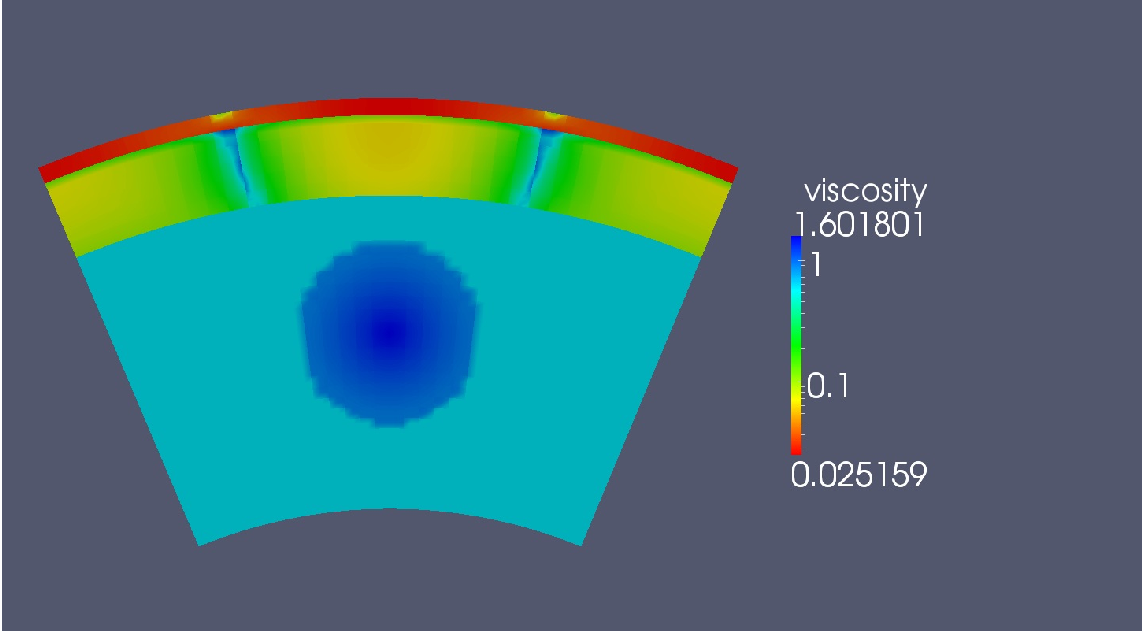
\includegraphics[height=70mm, width = 70mm]{true_visc.pdf}
}
\subfigure[]{
  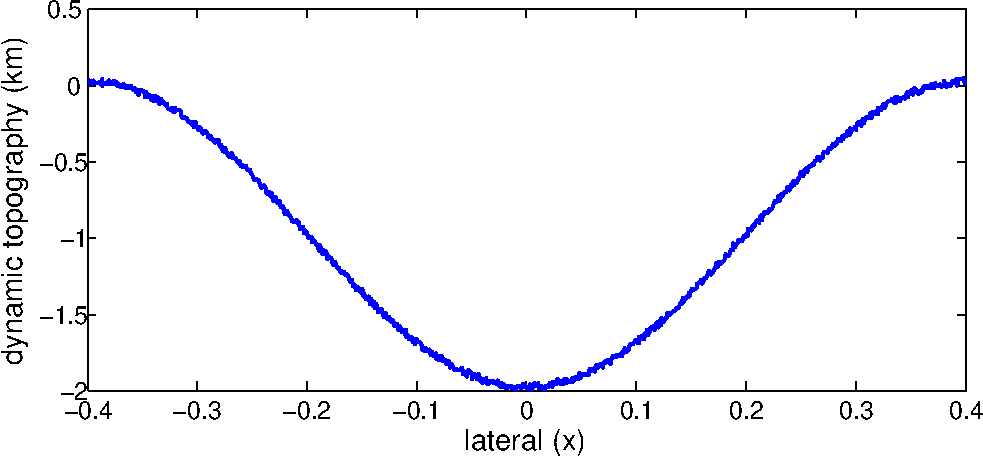
\includegraphics[height=70mm, width = 70mm]{topog_signal.pdf}
}
\caption{\mgnote{This Figure has more but continues to need improvement. First, is that you need to use or master a graphics package in which the material can be presented professionally, that is without distorting the aspect ratio. Second, on the left-hand side (a) You should show the temperature field as black contours ontop of the effective viscosity. On the right hand side you have two predictions, but only normal stress is shown. Either in this Figure or in an additional one, you need to show the velocity and normal stress is that obtained from the inverse model}(a) Effective viscosity (b)Dynamic topography (km) with 4 $\%$ noise}. 
\label{fig:viscosity}
\end{figure}
 
%The surface normal stress signal in Fig.\ref{fig:viscosity}b will be used as the observation for the inversions for the resulting cases. \mgnote{Why is this next sentance in the model setup section. This has nothing to do with model setup} Using this piece of data is advantageous because there is a strong response of the signal to the effective viscosity structure. 

\mgnote{You need to have a whole paragraph which describes the numerical methods (finite elements) with description of shape fundations and solver. You need to describe the mesh. You need to describe ay software (Rhea). You need to describe any issues with the optimization} \vrnote{done}
We will solve the forward problem using a finite element code that is highly scalable that makes  use of adaptive mesh refinement (AMR) \citep{rudi2015extreme}. Furthermore, we use Q2 elements for velocity while using first order discontinuous elements for pressure, to solve the Stokes flow problem.
\\mgnote{This is still insufficient -- actual size of elements, number of elements, library names, criteria used in AMR (i.e. error indicators), tolerance on solvers...}


\section*{Results}
With our computational method, we investigate how well we can recover the parameters with a combination of surface normal stress data and surface velocity  (Table \ref{table:inversions}).
\begin{sidewaystable}
\centering
	\begin{table}[H]
		\caption{Case study summary for inversions for multiple parameters with different pieces of data used. Note \textit{T} means topography, while \textit{v} means velocity data used. \mgnote{Thanks for running more cases. For those in which a variable is held fixed use Bold or underling to symbolize that fact and call this out here in the Caption. Use the same Style as in Chapter 4.}} % title of Table
		\centering  % used for centering table
		\begin{tabular}{c c c c c c} % centered columns (2 columns)
		\hline \hline                        %inserts double horizontal lines
		Case&n (Guess/Recov.) &$\gamma$ (Guess/Recov.)   &Activ. Energy (Guess/Recov.) &Iter. & Data  \\ [0.5ex] % inserts table
		%heading
		\hline                  % inserts single horizontal line
	        1 & 3.0  & $10^{-2}/10^{-1}$ &   1.0 & 2  & T\\
	        2 & 3.0  & $10^{-3}/10^{-1}$ & 1.0 & 2 & T\\
	        3 & 2.85/3.0  & $10^{-1}$ & 1.0  & 3 & T \\
	        4 & 2.0/3.0  & $10^{-1}$  & 1.0  & 5 & T \\
	        5 & 3.5/3.0  & $10^{-1}$   & 1.0  &3 & T \\
	        6 & 3.0  & $10^{-1}$  & 0.1/1.0  & 4 & T \\
	        7 & 3.0  & $10^{-1}$  & 0.4/1.0  & 4 & T \\
            8 & 2.0/3.0  & $10^{-3}/10^{-1}$ & 0.1/1.0  & 3 & T \\
	        9 & 2.8/3.0  & $10^{-1}$  & 1.0  & 3 & T \& v\\
	        10 & 3.0  & $10^{-2}/10^{-1}$ & 1.0  & 3 & T \& v\\
            11 & 3.0  & $10^{-1}$ & 0.1/1.0  & 3 & T \& v\\
            12 & 2.0/3.0  & $10^{-3}/10^{-1}$ & 1.0  & 3 & T \& v\\
            13 & 2.0/3.0  & $10^{-3}/10^{-1}$ & 0.1/1.0  & 3 & T \& v\\

                 
                \hline %inserts single line
		\end{tabular}
		\label{table:inversions} % is used to refer this table in the text
		\end{table}

\end{sidewaystable}
To test how well the new adjoint formulation of surface normal stress data works with respect to the recovery of the rheological parameters, we first focus on a single parameter, weak layer prefactor, strain rate exponent or activation energy. In Case 1, we infer the weakfactor of the top layer of the system, while keeping the other parameters fixed (strain rate exponent, yield stress and activation energy). We find that we are able to infer the correct weak layer prefactor within 2 iterations. 
\mgnote{An addition case is needed that starts with a $\gamma$ larger than the actual value.}
Furthermore, we test the independence of the initial guess to see if the inferred parameter is the same in Case 2. We find, similar to Case 1, that the recovered weak factor is $10^{-1}$, while the convergence to the true (synthetic value) is also 2 iterations (Fig.\ref{fig:topog_converge}a), 
suggesting that the physics of the system prefers this weakfactor.
\mgnote{I'm not sure what you mean. You need to be explicit}

We repeat similar case studies for the strain rate exponent, and activation energy. In Case 3, we keep the weak factor and activation energy fixed (effectively conditioning on the weak factor and activation energy), and find that we infer the correct strain rate exponent of 3.0 within 3 iterations, similar to the weafactor in Cases 1-2. Similarly, we test the independence of the initial guess of the strain rate exponent. We test two different guesses ($n=2.0,3.5$) that are smaller and larger than the initial guess of Case 3, and find in both Cases 4 and 5 that we can recover the true strain rate exponent within 3-4 iterations (Fig.\ref{fig:topog_converge}b), 
also suggesting that this particular model has a preferential amount of shear thinning needed to constrain the surface normal stress signal.
\mgnote{I don't know what this means . You need to be explicit.}

A parameter that we have not investigated in \citep{ratnaswamy2015adjoint} was the activation energy, which controls the amount of temperature dependence in the effective viscosity. We similarly follows the similar approach as we did for the weak factor and strain rate exponent (Cases 1-5) and infer the activation energy (as well as the independence) of that initial guess. We find in Case 6 (only inferring the activation energy), that  we are able to infer the activation energy, regardless of the in initial guess (Case 7) within 4 iterations (Fig.\ref{fig:topog_converge}c). 

While we were able to accurately infer the rheological parameters by themselves, it is important that we see how well this new adjoint formulation does when it comes to inferring multiple parameters using only surface normal stress data. We do so in Case 9 where we  infer the strain rate exponent, activation energy and weakfactor and find that we can infer all three parameters within 7 iterations, which possibly shows that as more parameters are inferred, the rate of convergence increases using only one piece of data.


The decrease in convergence when attempting to infer more parameters lends to to the question  of whether adding surface velocity would increase the convergence. To this end, we explore inferring the rheological parameters using both surface normal stress and surface velocity. We first infer individual parameters for both pieces of data to make sure that the correct value is attained. In Cases 9-11, we find that we correctly infer the strain rate exponent/weakfactor/activation energy within 3 iterations, suggesting that there may not be conflicts in using both data types. In Case 12, as we infer the strain rate exponent and weak factor, we also find that we infer the true value within 3 iterations. As a direct comparison to Case 8, we infer the strain rate exponent, weakfactor and activation energy in Case 13 and find that we not only are able to infer the correct values, but we do so in less iterations (4 iterations) as shown in Fig.\ref{fig:topog_converge}d,e,f.
\begin{figure}[H]
\centering
%\hspace{-0.2cm}\subfigure[]{
%\includegraphics[height=65mm,width=128mm]{visc_no_stress.jpg}%{mesh.pdf}
%}
\hspace{-0.6cm}\subfigure{
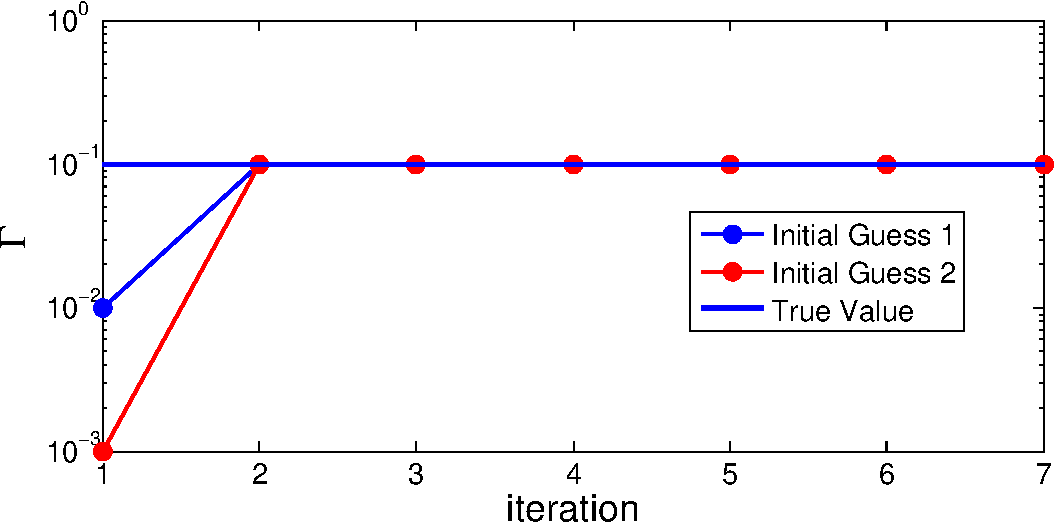
\includegraphics[height=35mm,width=48mm]{topog_gamm_only.pdf}%{mesh.pdf}
}
\hspace{-0.1cm}\subfigure{
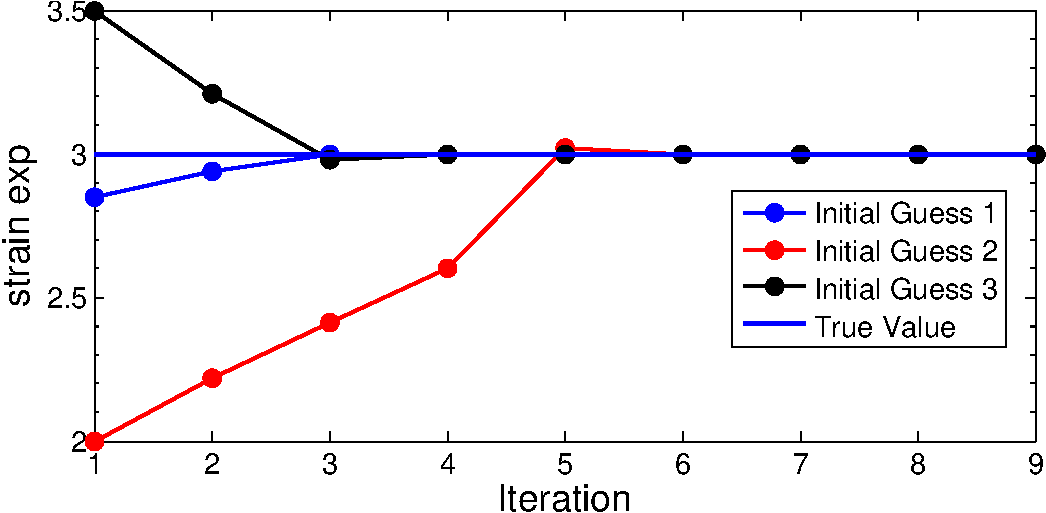
\includegraphics[height=35mm,width=48mm]{topog_strain_only.pdf}%{mesh.pdf}
}
\hspace{-0.1cm}\subfigure{
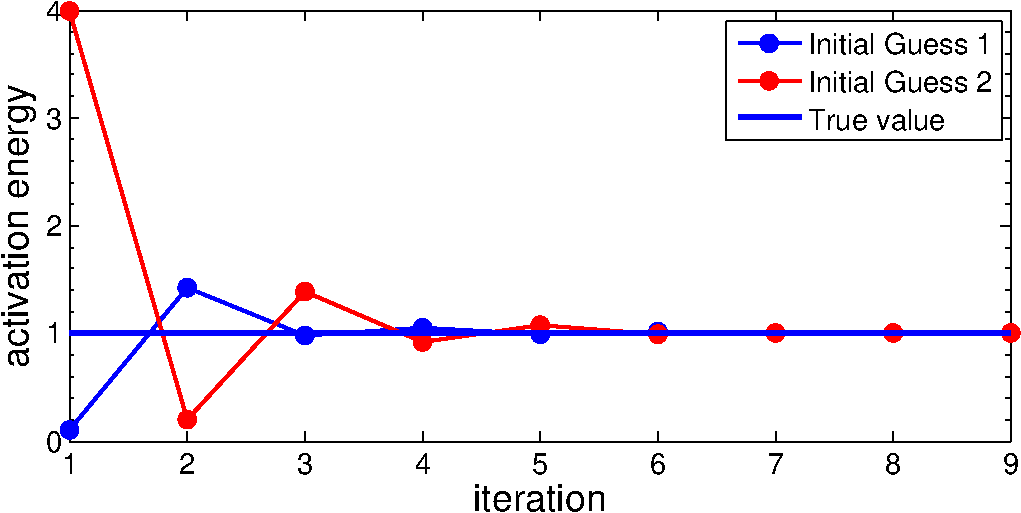
\includegraphics[height=35mm,width=48mm]{topog_activ_only.pdf}%{mesh.pdf}
}
\hspace{-1.8cm}\subfigure{
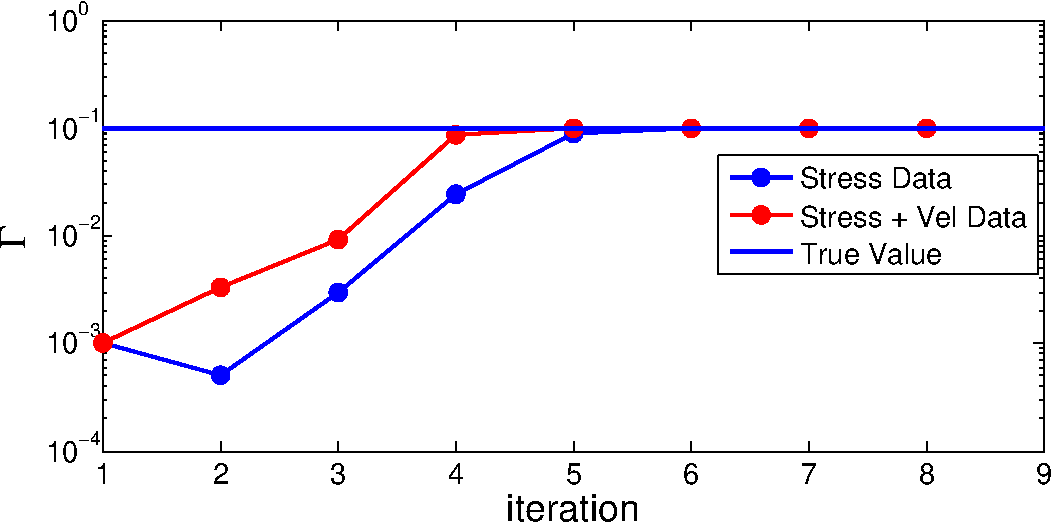
\includegraphics[height=35mm,width=48mm]{top_vel_gamma.pdf}%{mesh.pdf}
}
\hspace{-0.1cm}\subfigure{
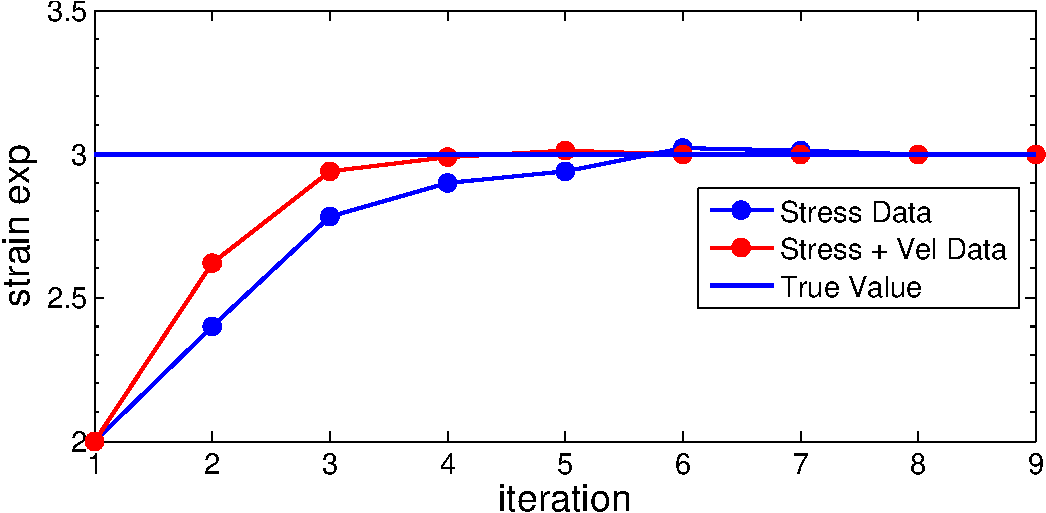
\includegraphics[height=35mm,width=48mm]{top_vel_strain.pdf}%{mesh.pdf}
}
\hspace{-0.1cm}\subfigure{
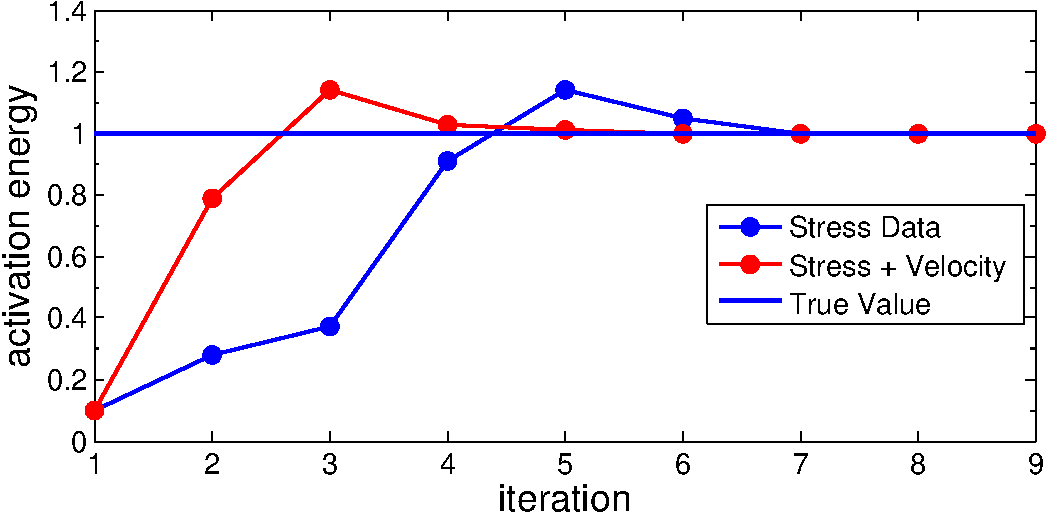
\includegraphics[height=35mm,width=48mm]{top_vel_activ.pdf}%{mesh.pdf}
}
%\hspace{-0.2cm}\subfigure[]{
%\includegraphics[height=35mm,width=58mm]{um_chap4.pdf}%{mesh.pdf}
%}
\caption{ \mgnote{This Figure looks messy and unprofessional. I think this is caused by your Figure in the upper left which has a smaller width than the others. Each Subfigure needs a letter label. The Fonts for the Labels needs to be larger}(a)  Cases 1 and 2 (inference for weakfactor with only normal stress data) (b)Cases 3-5 (inference for strain rate exponent with only normal stress data) (c) Cases 6 and 7 (inference for activation energy with only normal stress data) (d) Weakfactor comparison between cases 8 and 13 (e)Strain rate exponent comparison between cases 8 and 13 (f) Activation energy comparison between cases 8 and 13 }
\label{fig:topog_converge}
\end{figure}







	




\section*{Discussion}

\mgnote{This first figure just repeats what you presented in your results. Move beyond the superficial and explain why and what are the limitatitations, advantages, prospects, what has been done before. That is what discussion is.}
We were able to infer various rheological parameters for the sinking mass anomaly using this new adjoint formulation. We show that in Cases 1-2, we can correctly infer the weak layer prefactor, (independent of the initial guess), within 3 iterations. We similarly find that we can infer the strain rate exponent (Cases 3-5) and activation energy (Cases 6-7) within 4-5 iterations, independent of the initial guess.  Furthermore, we demonstrate that using both surface velocity and surface normal stress can potentially accelerate the convergence of inversions as shown between Case 8 and 13.

 While we were able to implement and prove the validity of using the surface normal stress in the adjoint formulation, there still are issues in applying this method to subduction zones. One of these issues lies in the large variations in viscosity and the boundary conditions on the surface \citep{crameri2017dynamical}. The problem is that there are large dynamic topography near the trench that exceed 10km in forward models, which is certainly not found in the observations. Therefore, the adjoint formulation with surface normal stress will not work when no forward model is able to produce reasonable short wavelength topographic signals. 
 
 
  The problematic issue of large topographic magnitudes can be traced to the large variations in viscosity of the forward model between plate and the weakzone ($\mathcal{O}(10^6)$). We find that when the viscosity variations are reduced, the magnitude of the topography was also reduced. However, this also caused an increase in the fore-bulge. Additionally, when using a sticky-air surface (weak viscosity layer at the surface), we find that the we could reduce the amplitude of the topography signal at the trench. The sticky-air method brings an added complication of measuring the topography due to the interface between the sticky-air layer and the oceanic plates. It is certainly clear from those investigations that to remedy the large trench depths requires a different formulation of the effective viscosity and/or surface boundary conditions. However, after the issue of large topographic signals is resolved, the use of the adjoint with surface normal stress can be readily used.

\bibliography{references}


\appendix
\section{Gradient and Hessian Tests}
\subsection{Cases 1 and 2}
\begin{table}[H]
		\caption{Inversion statistics for $\gamma_{\text{guess}}= 10^{-2}$} % title of Table
		\centering  % used for centering table
		\begin{tabular}{c c c } % centered columns (2 columns)
		\hline \hline                        %inserts double horizontal lines
 		$Iteration$&$\mathcal H$ &$|\mathcal G|$   \\ [0.5ex] % inserts table
		%heading
		\hline                  % inserts single horizontal line
                $1$&$2.02\cdot 10^{9}$&$3.675\cdot 10^{10}$   \\
		$2$&$3.47\cdot 10^{10}$&$2.948\cdot 10^{9}$   \\
                $3$&$4.95\cdot 10^{10}$&$1.899\cdot 10^{8}$   \\
		$4$&$5.46\cdot 10^{10}$&$9.91\cdot 10^{6}$   \\
		$5$&$5.72\cdot 10^{10}$&$5.06\cdot 10^{5}$   \\

                \hline %inserts single line
		\end{tabular}
		\label{table:gradcheck1} % is used to refer this table in the text
		\end{table}
 

\begin{table}[H]
		\caption{Inversion statistics for $\gamma_{\text{guess}}= 10^{-3}$} % title of Table
		\centering  % used for centering table
		\begin{tabular}{c c c } % centered columns (2 columns)
		\hline \hline                        %inserts double horizontal lines
 		$Iteration$&$\mathcal H$ &$|\mathcal G|$   \\ [0.5ex] % inserts table
		%heading
		\hline                  % inserts single horizontal line
                $1$&$1.248\cdot 10^{8}$&$8.452\cdot 10^{10}$   \\
		$2$&$5.53\cdot 10^{10}$&$3.7718\cdot 10^{9}$   \\
                $3$&$5.775\cdot 10^{10}$&$1.531\cdot 10^{8}$   \\
		$4$&$5.917\cdot 10^{10}$&$9.91\cdot 10^{6}$   \\
		$5$&$6.002\cdot 10^{10}$&$7.97\cdot 10^{5}$   \\
	        $6$&$6.05\cdot 10^{10}$&$6.374\cdot 10^{5}$   \\
        	$7$&$6.08\cdot 10^{10}$&$5.06\cdot 10^{4}$   \\
        
                \hline %inserts single line
		\end{tabular}
		\label{table:gradcheck2} % is used to refer this table in the text
		\end{table}

\subsection{Cases 3-5}
\begin{table}[H]
		\caption{Inversion statistics for $n_{\text{guess}}= 2.85$} % title of Table
		\centering  % used for centering table
		\begin{tabular}{c c c } % centered columns (2 columns)
		\hline \hline                        %inserts double horizontal lines
 		$Iteration$&$\mathcal H$ &$|\mathcal G|$   \\ [0.5ex] % inserts table
		%heading
		\hline                  % inserts single horizontal line
                $1$&$3.977\cdot 10^{12}$&$1.717\cdot 10^{11}$   \\
		$2$&$3.0604\cdot 10^{12}$&$8.663\cdot 10^{10}$   \\
                $3$&$2.104\cdot 10^{12}$&$3.356\cdot 10^{9}$   \\
		$4$&$2.057\cdot 10^{12}$&$4.461\cdot 10^{8}$   \\
		$5$&$2.0638\cdot 10^{12}$&$6.985\cdot 10^{7}$   \\
		$6$&$2.06281\cdot 10^{12}$&$1.044\cdot 10^{7}$   \\
		$7$&$2.06296\cdot 10^{12}$&$1.567\cdot 10^{6}$   \\
 		$8$&$2.06294\cdot 10^{12}$&$2.342\cdot 10^{5}$   \\
		$9$&$N/A$&$3.5047\cdot 10^{4}$   \\

                \hline %inserts single line
		\end{tabular}
		\label{table:gradcheck3} % is used to refer this table in the text
		\end{table}
 

\begin{table}[H]
		\caption{Inversion statistics for $n_{\text{guess}}= 2.0$} % title of Table
		\centering  % used for centering table
		\begin{tabular}{c c c } % centered columns (2 columns)
		\hline \hline                        %inserts double horizontal lines
 		$Iteration$&$\mathcal H$ &$|\mathcal G|$   \\ [0.5ex] % inserts table
		%heading
		\hline                  % inserts single horizontal line
                $1$&$2.7665\cdot 10^{13}$&$3.488\cdot 10^{12}$   \\
		$2$&$3.944\cdot 10^{13}$&$2.912\cdot 10^{12}$   \\
                $3$&$3.092\cdot 10^{13}$&$1.257\cdot 10^{12}$   \\
		$4$&$8.617\cdot 10^{12}$&$2.675\cdot 10^{11}$   \\
		$5$&$1.797\cdot 10^{12}$&$1.1778\cdot 10^{10}$   \\
		$6$&$2.146\cdot 10^{12}$&$3.647\cdot 10^{9}$   \\
		$7$&$2.0496\cdot 10^{12}$&$5.832\cdot 10^{8}$   \\
 		$8$&$2.0655\cdot 10^{12}$&$1.137\cdot 10^{8}$   \\
		$9$&$2.06245\cdot 10^{12}$&$2.159\cdot 10^{7}$   \\
                \hline %inserts single line
		\end{tabular}
		\label{table:gradcheck4} % is used to refer this table in the text
		\end{table}


\begin{table}[H]
		\caption{Inversion statistics for $n_{\text{guess}}= 3.5$} % title of Table
		\centering  % used for centering table
		\begin{tabular}{c c c } % centered columns (2 columns)
		\hline \hline                        %inserts double horizontal lines
 		$Iteration$&$\mathcal H$ &$|\mathcal G|$   \\ [0.5ex] % inserts table
		%heading
		\hline                  % inserts single horizontal line
                $1$&$3.658\cdot 10^{11}$&$3.1396\cdot 10^{11}$   \\
		$2$&$1.2446\cdot 10^{12}$&$1.76443\cdot 10^{11}$   \\
                $3$&$2.64779\cdot 10^{12}$&$1.351\cdot 10^{11}$   \\
		$4$&$2.03321\cdot 10^{12}$&$6.92\cdot 10^{9}$   \\
		$5$&$2.06992\cdot 10^{12}$&$1.386\cdot 10^{9}$   \\
		$6$&$2.06271\cdot 10^{12}$&$2.525\cdot 10^{8}$   \\
		$7$&$2.06406\cdot 10^{12}$&$6.143\cdot 10^{7}$   \\
 		$8$&$2.06372\cdot 10^{12}$&$2.221\cdot 10^{7}$   \\
		$9$&$2.06381\cdot 10^{12}$&$7.9271\cdot 10^{6}$   \\
                \hline %inserts single line
		\end{tabular}
		\label{table:gradcheck5} % is used to refer this table in the text
		\end{table}
        
 \begin{table}[H]
		\caption{Gradient check for activation energy with $E_a^0=4.0$} % title of Table
		\centering  % used for centering table
		\begin{tabular}{c c c } % centered columns (2 columns)
		\hline \hline                        %inserts double horizontal lines
		$iteration$&$\mathcal{G}_{Adjoint}$&$\mathcal{G}_{FD}$  \\ [0.5ex] % inserts table
		%heading
		\hline                  % inserts single horizontal line
		$1$ & $3.812 \cdot 10^{8}$ &$3.892\cdot 10^{8}$  \\
	 	$2$ & $-4.622\cdot 10^{7}$ &$-4.632\cdot 10^{7}$   \\
	        $3$ &$2.114 \cdot 10^{6}$ &$2.101\cdot 10^{6}$   \\
		$4$ &$-5.44\cdot 10^{5}$ &$-5.342\cdot 10^{5}$   \\
		$5$ &$6.9301 \cdot 10^{4}$ &$6.922\cdot 10^{4}$   \\
		$6$ &$-5.10 \cdot 10^{4}$ &$-5.102\cdot 10^{4}$ \\
		$7$ &$2.110 \cdot 10^{4}$ &$2.115\cdot 10^{4}$ \\
		$8$ &$-1.01 \cdot 10^{4}$ &$-1.02\cdot 10^{4}$ \\
                

                \hline %inserts single line
		\end{tabular}
		\label{table:parameters} % is used to refer this table in the text
		\end{table}       

\end{document}
